\documentclass[10pt, a4paper]{article}

\usepackage[paper=a4paper, left=1.5cm, right=1.5cm, bottom=1.5cm, top=3.5cm]{geometry}
\usepackage[utf8]{inputenc}
\usepackage[spanish]{babel}
\usepackage{caratula}
\usepackage{framed}
\usepackage{ulem}
\usepackage[pdftex]{graphicx}
\usepackage{float}
\usepackage{listings}
\usepackage{hyperref}
\usepackage{amsmath}
\usepackage{amssymb}
\usepackage{algorithm}
\usepackage[noend]{algpseudocode}


%Datos para la caratula
\materia{Base de Datos}

\titulo{Trabajo Práctico 1}


\integrante{Gasco, Emilio}{171/12}{gascoe@gmail.com}
\integrante{Rago, Pablo Diego}{239/10}{p4blo.r@gmail.com}
\integrante{Tolchinsky, Lucas}{591/07}{lucas.tolchinsky@gmail.com}
\integrante{Vallejo, Nicolás Agustín}{500/10}{nicopr08@gmail.com}

\fecha{8 de Mayo de 2015}

\begin{document}
	\maketitle
	\tableofcontents
	\newpage
	\section{Diagrama Entidad-Relación}
\subsection{Diagrama Entidad-Relación}
\begin{figure}[H]
   \begin{center}
   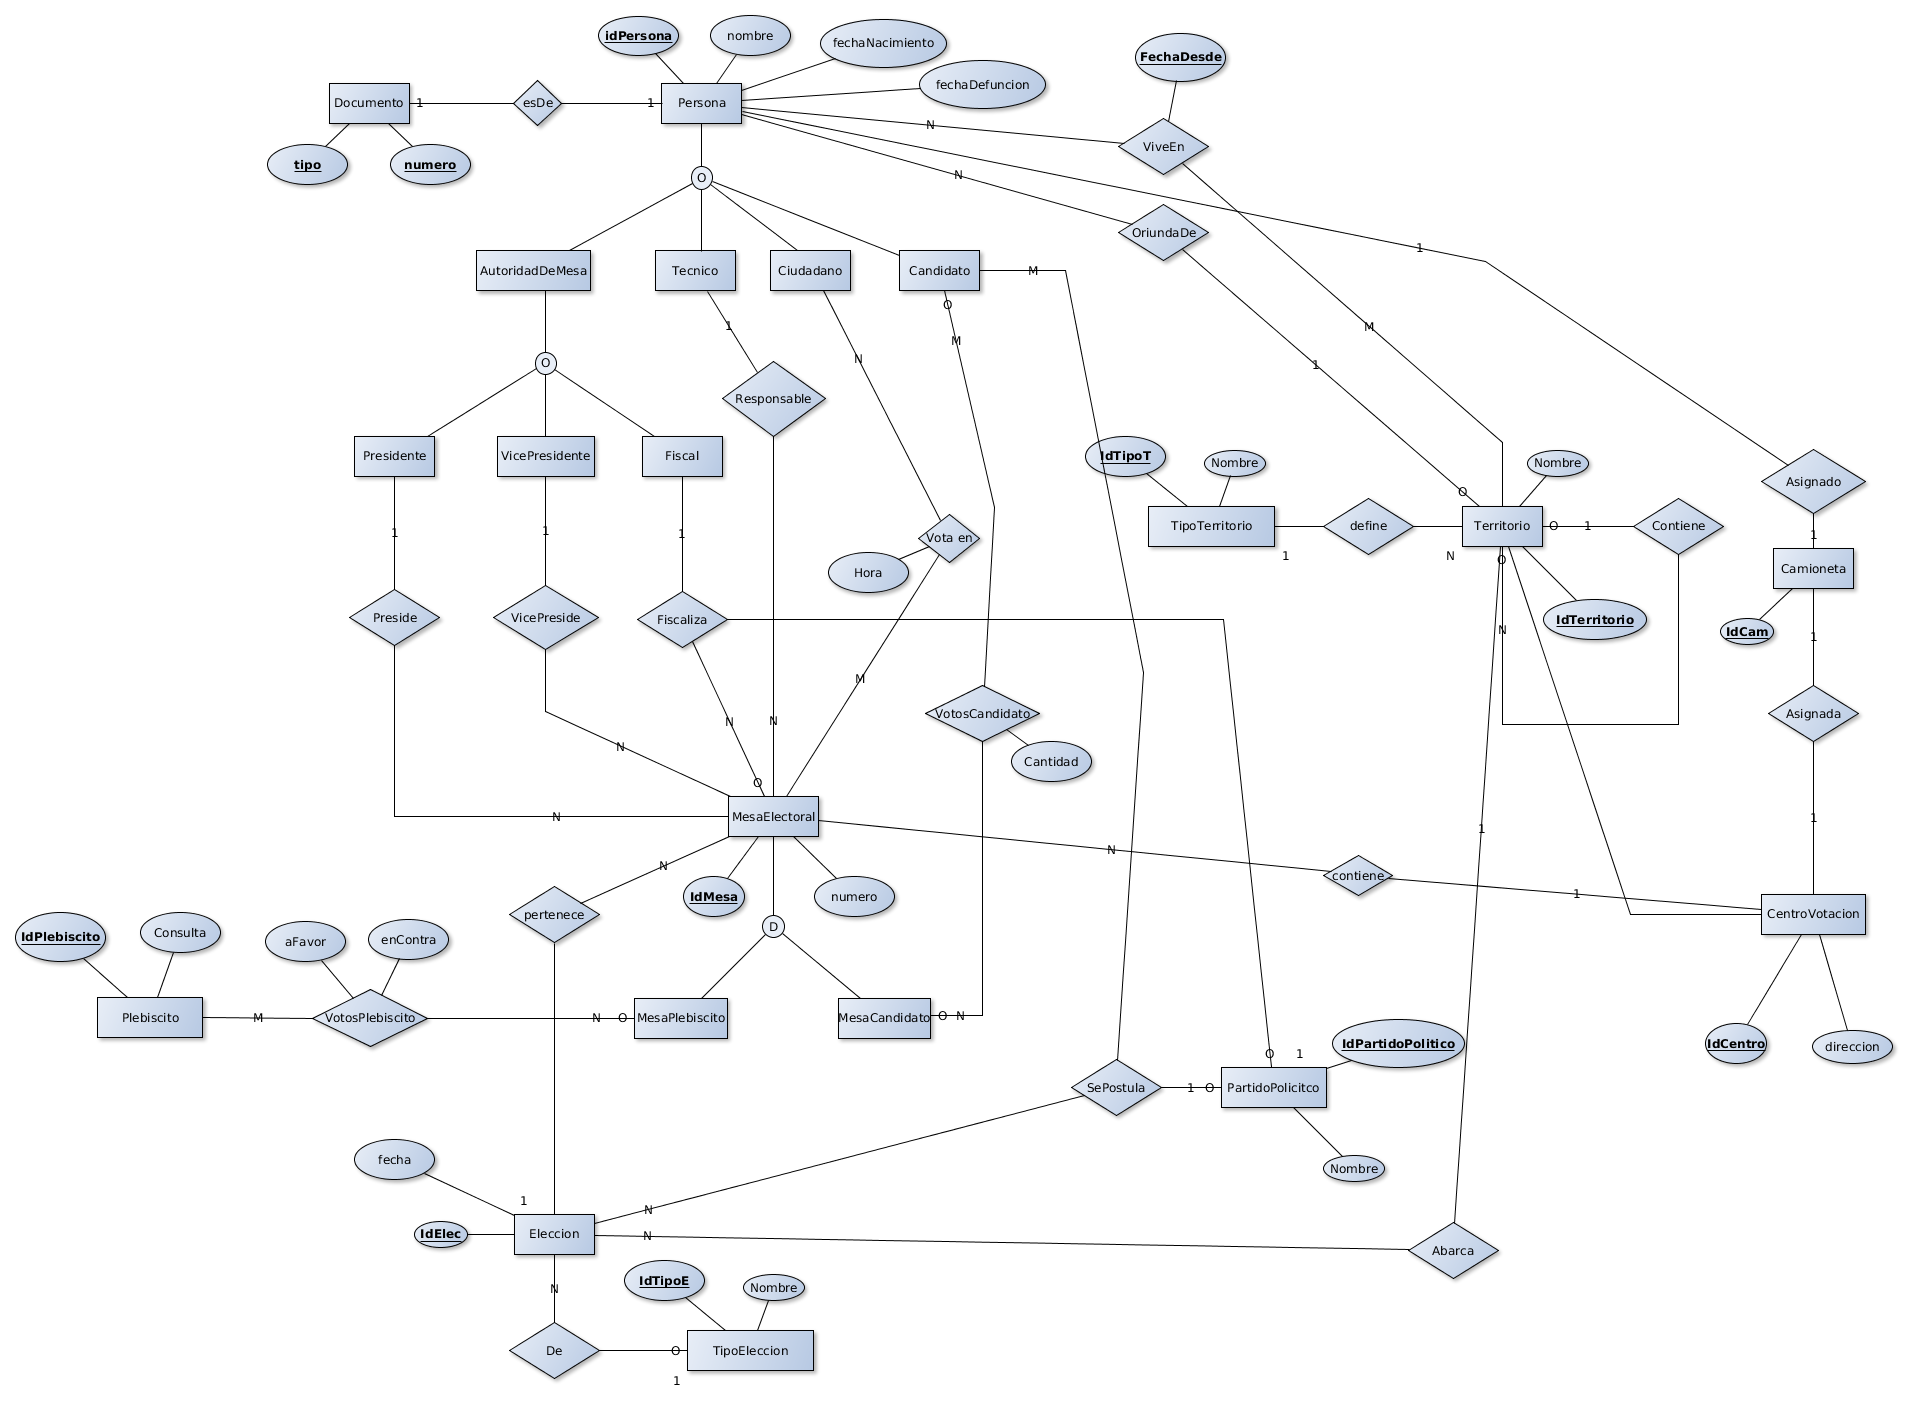
\includegraphics[angle=90,scale=0.32]{graphics/der.png}
   \caption{\textbf{Diagrama Entidad-Relación}}
   \label{fig:der}
   \end{center}
\end{figure}

\subsection{Restricciones Adicionales}

\subsubsection{Sobre los atributos}

\begin{itemize}
	\item{El número del Documento tiene que ser mayor a cero}.
	\item{El tipo del Documento tiene que ser alguno de los siguientes:
		\begin{itemize}
			\item{DNI}
			\item{CI}
			\item{LE}
			\item{LC}
		\end{itemize}
	}	
	\item{El atributo cantidad de la relación VotosCandidato tiene que ser mayor o igual a cero}

	\item{El atributo nombre de TipoTerritorio debe ser alguno de los siguientes y no se pueden repetir:
	  \begin{itemize}
	  	\item{País}
	  	\item{Provincia}
	  	\item{Localidad}
	  	\item{Ciudad}
	  \end{itemize}
	 }
	\item{El número de la MesaElectoral tiene que ser mayor a cero.}
	\item{Los  atributos aFavor y enContra de la relación VotosPlebiscito  tienen que ser mayor o igual a 0.}
	\item{El atributo fechaNacimiento no puede ser posterior al atributo fechaDefunción.}
\item{El atributo nombre de TipoEleccion debe ser alguno de los siguientes y no se pueden repetir:
	\begin{itemize}
		\item{Presidencial}
		\item{Gobernador}
		\item{Intendente}
		\item{Plebiscito}
	\end{itemize}
}

\item{Territorios sólo pueden contener a territorios más chicos:
\begin{itemize}
	\item{Un País sólo puede contener Provincias.}
	\item{Una Provincia sólo puede contener Localidades.}
	\item{Una Localidad sólo puede contener Ciudades.}
	\item{Una Ciudad no puede contener nada.}
\end{itemize}
}
\item{Sólo se puede ser oriundo de una ciudad.}

\item{Sólo los Territorios con TipoTerritorio de nombre "Ciudad" pueden participar de la relación OriundoDe.}
\item{Votar en las elecciones que corresponden según territorio.}

\item{Para que un Ciudadano pueda participar en VotosCandidato o VotosPlebiscito con la MesaElectoral correspondiente, ésta debe pertenecer a una Eleccion que abarque un Territorio el cual debe ser igual o contiene en algún nivel al Territorio en el cual el Ciudadano ViveEn en el momento de la elección.\footnote{Quien participa de ViveEn es Persona, no Ciudadano. Nos estamos refiriendo a la Persona correspondiente a dicho Ciudadano.}
}

%Presentarse como candidato para la elección de algún cargo.

\item{Para que un Candidato pueda participar de SePostula con un PartidoPolítico en una Eleccion, el Territorio que esta última abarca debe ser igual o contener en algún nivel al Territorio en el cual el Candidato debe participar en ViveEn\footnote{Idem [1] pero para Candidato.} con una fechaDesde mayor a los X años.
}

%Solamente reciben votos los candidatos que se presentan a la elección.

\item{Para que un Candidatos puede participar de VotosCandidato con MesaCandidato, debe participar en SePostula con la Elección a la cual la MesaElectoral pertenece.
}

%Si el Partido Político tiene fiscales, tiene que postularse.

\item{Para que PartidoPolítico participe de fiscaliza con una MesaElectoral, debe participar en sePostula con un Candidato en una Elección que contenga esa MesaElectoral.}

\item{Dentro de una Elección, los números de MesaElectoral no se pueden repetir.}

\item{Para cada elección, una Persona sólo puede ser Presidente, VicePresidente, Fiscal, Candidato o Técnico de manera disjunta.}


\item{Ciudadanos sólo pueden votarEn una única MesaElectoral por Elección.}

\item{No puede pasar que para una elección haya por lo menos una  MesasElectorales y por lo menos una MesaPlebiscito.}

\item{No hay más votos que votantes}

\item{Para cada MesaCandidato, la sumatoria de cantidad en cada tupla de VotoCandidato debe ser menor igual a la cantidad de tuplas en la relación VotaEn entre MesaElectoral y Ciudadano.}

\item{Para cada MesaPlebiscito, la sumatoria de aFavor y enContra en cada tupla de VotoPlebiscito debe ser menor igual a la cantidad de tuplas en la relación VotaEn entre MesaElectoral y Ciudadano.}

\item{Mayor de 16 para votar.}

\item{Para que una Persona sea Ciudadano tiene que tener más de 16 años.}

\item{Los muertos no votan}

\item{Para que un Ciudadano participe en VotaEn con una MesaElectoral, no debe tener fecha de defunción anterior a la fecha de la Elección correspondiente a esa Mesa.}

\item{No puede haber 2 o más  elecciones con misma fecha y mismo TipoEleccion para mismo Terrritorio.}

\end{itemize}


\subsection{Consideraciones}

\subsubsection{Acerca de las afiliaciones a los partidos políticos}

\begin{itemize}
\item{Hemos decidido no modelar las afiliaciones de las personas a los partidos políticos, no sólo porque podrían ser muchas tuplas, sino que no nos parece un aspecto central del problema a modelar.}

\item{Consideramos que las afiliaciones a los partidos políticos de fiscales y candidatos se entienden por sus participaciones en fiscaliza y sePostula, respectivamente.}
\end{itemize}

\subsubsection{Sobre el impedimento para postularse según lugar de nacimiento.}

\begin{itemize}
\item{Sabemos que ciertos cargos requieren que un candidato haya nacido en el territorio correspondiente a la elección, como por ejemplo la elección de Presidente.Sin embargo, esto no es requerido para todos los cargos políticos y por ese motivo no forzamos esa restricción.}
\end{itemize}

	\newpage
	\section{Modelo Relacional}

\textbf{Eleccion}(idEleccion, fecha, idTipoEleccion, idTerritorio)\\
  PK = CK = \{idEleccion\}\\
  FK = \{idTipoEleccion, idTerritorio\}\\
\\
\textbf{TipoEleccion}(idTipoEleccion, nombre)\\
  PK = CK = \{idTipoEleccion\}\\
\\
\textbf{MesaElectoral}(idMesaElectoral, numero, idPresidente, idVicePresidente, idTecnico, idCentroVotacion, idEleccion)\\
  PK = CK = \{idMesaElectoral\}\\
  FK = \{idPresidente, idVicePresidente, idFiscal, idTecnico, idCentroVotacion, idEleccion\}\\
\\
\textbf{MesaPlebiscito}(idMesaElectoral)\\
  PK = CK = FK = \{idMesaElectoral\}\\
\\
\textbf{MesaCandidato}(idMesaElectoral)\\
  PK = CK = FK = \{idMesaElectoral\}\\
\\
\textbf{Plebiscito}(idPlebiscito, Consulta)\\
  PK = CK = \{idPlebiscito\}\\
\\
\textbf{VotosPlebiscito}(idPlebiscito, idMesaElectoral, aFavor, enContra)\\
  PK = CK = \{(idPlebiscito, idMesaElectoral)\}\\
  FK = \{idPlesbiscito, idMesaElectoral\}\\
\\
\textbf{CentroVotacion}(idCentroVotacion, direccion, idTerritorio, idCamioneta)\\
  PK = CK = \{idCentroVotacion\}\\
  FK = \{idTerritorio, idCamioneta\}\\
\\
\textbf{Camioneta}(idCamioneta,patente idPersona)\\
  PK = CK = \{idCamioneta\}\\
  FK = \{idPersona\}\\
\\
\textbf{PartidoPolitico}(idPartidoPolitico, nombre)\\
  PK = CK = \{idPartidoPolitico\}\\
\\
\textbf{VotosCandidato}(idMesaElectoral, idPersona, cantidad)\\
  PK = CK = \{(idMesaElectoral, idPersona)\}\\
  FK = \{idMesaElectoral, idPersona\}\\
\\
\textbf{Documento}(tipo, numero, idPersona)\\
  PK = CK = \{(tipo, numero)\}\\
  FK = \{idPersona\}\\
\\
\textbf{Persona}(idPersona, nombre, fechaNacimiento, fechaDefuncion, idTerritorio)\\
  PK = CK = \{idPersona\}\\
  FK = \{idTerritorio\}\\
\\
\textbf{ViveEn}(idPersona, idTerritorio, fechaDesde)\\
  PK = CK = \{(idPersona, idTerritorio, fechaDesde)\}\\
  FK = \{idPersona, idTerritorio\}\\
\\
\textbf{Tecnico}(idPersona)\\
  PK = CK = FK = \{idPersona\}\\
\\
\textbf{Ciudadano}(idPersona)\\
  PK = CK = FK = \{idPersona\}\\
\\
\textbf{Candidato}(idPersona)\\
  PK = CK = FK = \{idPersona\}\\
\\
\textbf{AutoridadDeMesa}(idPersona)\\
  PK = CK = FK = \{idPersona\}\\
\\
\textbf{Presidente}(idPersona)\\
  PK = CK = FK = \{idPersona\}\\
\\
\textbf{VicePresidente}(idPersona)\\
  PK = CK = FK = \{idPersona\}\\
\\
\textbf{Fiscal}(idPersona)\\
  PK = CK = FK = \{idPersona\}\\
\\
\textbf{VotaEn}(idCiudadano, idMesaElectoral, hora)\\
  PK = CK = \{(idCiudadano, idMesaElectoral)\}\\
  FK = \{idCiudadano, idMesaElectoral\}\\
\\
\textbf{SePostula}(idEleccion, idCandidato, idPartidoPolitico)\\
  PK = \{(idEleccion, idCandidato)\}\\
  CK = \{(idEleccion, idCandidato)\}\\
  FK = \{idEleccion, idCandidato, idPartidoPolitico\}\\
\\
\textbf{Fizcaliza}(idFiscal, idMesaElectoral, idPartidoPolitico)\\
  PK = \{(idMesaElectoral, idFiscal)\}\\
  CK = \{(idMesaElectoral, idFiscal), (idMesaElectoral, idPartidoPolitico)\}\\
  FK = \{idMesaElectoral, idFiscal, idPartidoPolitico\}\\
\\
\textbf{Territorio}(idTerritorio, nombre, idTipoTerritorio, idTerritorioPadre)\\
  PK = CK = \{idTerritorio\}
  FK = \{idTipoTerritorio, idTerritorioPadre\}\\
\\
\textbf{TipoTerritorio}(idTipoTerritorio, nombre)\\
  PK = CK = \{idTipoTerritorio\}\\	
	\newpage
	\section{Implementación}


\subsection{Triggers}

\subsubsection{Una persona sólo puede ser oriunda de una ciudad.}

\begin{verbatim}
CREATE OR REPLACE FUNCTION OriundaDeCiudad() RETURNS TRIGGER AS $$
    BEGIN
    IF (SELECT count(*) 
        FROM Territorio 
        WHERE idTerritorio=NEW.idTerritorio AND idTipoTerritorio=3) = 0 
        THEN
            RAISE EXCEPTION 'Solo puede ser oriundo de una ciudad';              
        ELSE
            RETURN NEW;
    END IF;
    RETURN NULL;
    END;
$$ LANGUAGE plpgsql;


CREATE TRIGGER CheckInsertPersona
    BEFORE INSERT ON Persona
    FOR EACH ROW EXECUTE PROCEDURE OriundaDeCiudad();

\end{verbatim}

\subsubsection{No se puede agregar dos veces el mismo candidato en VotosCandidatos para la misma mesa.}
\begin{verbatim}

CREATE OR REPLACE FUNCTION checkVotosCandidato() RETURNS TRIGGER AS $$
    BEGIN
    IF (SELECT count(*) 
        FROM MesaElectoral M 
        INNER JOIN Eleccion E ON M.idEleccion = E.idEleccion
        INNER JOIN SePostula S on E.idEleccion =  S.idEleccion
        WHERE S.idCandidato = NEW.idCandidato 
        AND M.idMesaElectoral = NEW.idMesaElectoral ) = 0
        THEN
            RAISE EXCEPTION 
            'El candidato se ha postulado para la eleccion de la 
            Mesa';              
        ELSE
            RETURN NEW;
    END IF;
    RETURN NULL;
    END;
$$ LANGUAGE plpgsql;


CREATE TRIGGER CheckInsertVotosCandidato
    BEFORE INSERT ON VotosCandidato
    FOR EACH ROW EXECUTE PROCEDURE checkVotosCandidato();


CREATE TRIGGER CheckUpdateVotosCandidato
    BEFORE UPDATE ON VotosCandidato
    FOR EACH ROW EXECUTE PROCEDURE checkVotosCandidato();

\end{verbatim}

\subsubsection{Para una elección dada, una persona no puede ser autoridad de mesa en más de una mesa electoral.}
\begin{verbatim}
CREATE OR REPLACE FUNCTION  AutoridadesEleccion(idE int) 
    RETURNS TABLE (idPersona int) AS $$
BEGIN
    RETURN query 
        SELECT idPresidente from MesaElectoral Where idEleccion = idE;
    RETURN query 
        SELECT idVicePresidente from MesaElectoral Where idEleccion = idE;
    RETURN query 
        SELECT idTecnico from MesaElectoral Where idEleccion = idE;
    RETURN query 
        SELECT idFiscal 
        from Fiscaliza F 
        INNER JOIN MesaElectoral M ON F.idMesaElectoral = M.idMesaElectoral 
        WHERE M.idEleccion = idE;
END;
$$ LANGUAGE plpgsql;

CREATE OR REPLACE FUNCTION checkAutoridad() RETURNS TRIGGER AS $$
    BEGIN
    IF ( NEW.idPresidente IN ( SELECT AutoridadesEleccion(NEW.idEleccion) ) OR
        NEW.idVicePresidente IN ( SELECT AutoridadesEleccion(NEW.idEleccion) ) OR
        NEW.idTecnico IN ( SELECT AutoridadesEleccion(NEW.idEleccion) ) )
        THEN
            RAISE EXCEPTION 'Alguna de las autoridades seleccionadas para esta 
            mesa ya es Autoridad para otra mesa';
        ELSE
            RETURN NEW;
    END IF;
    RETURN NULL;
    END;
$$ LANGUAGE plpgsql;

CREATE TRIGGER CheckInsertMesaElectoral
    BEFORE INSERT ON MesaElectoral
    FOR EACH ROW EXECUTE PROCEDURE checkAutoridad();

CREATE TRIGGER CheckUpdateMesaElectoral
    BEFORE UPDATE ON MesaElectoral
    FOR EACH ROW EXECUTE PROCEDURE checkAutoridad();

\end{verbatim}

\subsubsection{No puede haber fiscales de partidos que no participen en la elección ni tampoco fiscales en mesas inexistentes.}
\begin{verbatim}
CREATE OR REPLACE FUNCTION checkPartidoDeFiscalPostulado() RETURNS TRIGGER AS $$
    BEGIN
    IF (SELECT count(*) 
        FROM MesaElectoral M 
        INNER JOIN Eleccion E ON M.idEleccion = E.idEleccion
        INNER JOIN SePostula S on E.idEleccion =  S.idEleccion
        WHERE M.idMesaElectoral = NEW.idMesaElectoral 
            AND S.idPartidoPolitico = NEW.idPartidoPolitico) = 0 
        THEN
            RAISE EXCEPTION 'El partido a fiscalizar no esta postulado o la Mesa
            no existe';              
        ELSE
            RETURN NEW;
    END IF;
    RETURN NULL;
    END;
$$ LANGUAGE plpgsql;

CREATE TRIGGER CheckInsertPartidoDeFiscalPostuladoFiscaliza
    BEFORE INSERT ON Fiscaliza 
    FOR EACH ROW EXECUTE PROCEDURE checkPartidoDeFiscalPostulado();


CREATE TRIGGER CheckUpdatePartidoDeFiscalPostuladoFiscaliza
    BEFORE UPDATE ON Fiscaliza 
    FOR EACH ROW EXECUTE PROCEDURE checkPartidoDeFiscalPostulado();
\end{verbatim}

\subsubsection{Un fiscal no puede ser a la vez autoridad de mesa en la elección.}

\begin{verbatim}
CREATE OR REPLACE FUNCTION checkFiscalNoEsAutoridadParaEleccion() RETURNS TRIGGER AS $$
    DECLARE
    idE INT;
    BEGIN
    SELECT idEleccion 
    INTO idE 
    FROM MesaElectoral WHERE idMesaElectoral = NEW.idMesaElectoral;
    IF NEW.idFiscal IN  (SELECT AutoridadesEleccion(idE)) THEN
        RAISE EXCEPTION 'El fiscal ya es autoridad de Mesa o la Mesa no existe';
    ELSE
        RETURN NEW;
    END IF;
    RETURN NULL;
    END;
$$ LANGUAGE plpgsql;


CREATE TRIGGER CheckInsertNoEsAutoridadParaEleccionFiscaliza
    BEFORE INSERT ON Fiscaliza 
    FOR EACH ROW EXECUTE PROCEDURE checkFiscalNoEsAutoridadParaEleccion();


CREATE TRIGGER CheckUpdateNoEsAutoridadParaEleccionFiscaliza
    BEFORE UPDATE ON Fiscaliza 
    FOR EACH ROW EXECUTE PROCEDURE checkFiscalNoEsAutoridadParaEleccion();
\end{verbatim}

\subsubsection{Sólo personas vivas y mayores de 16 años pueden ser autoridades de mesa.}
\begin{verbatim}
CREATE OR REPLACE FUNCTION checkAutoridadDeMesa() RETURNS TRIGGER AS $$
    DECLARE
    edad INT;
    BEGIN
    SELECT date_part('year',age(fechaNacimiento))  
    INTO edad 
    FROM Persona 
    WHERE idPersona = NEW.idPersona AND fechaDefuncion IS NULL ;
    IF edad < 16 
        THEN
            RAISE EXCEPTION 'Hay que tener mas de 16 años y estar vivo para ser 
            autoridad de Mesa';
        ELSE
            RETURN NEW;
    END IF;
    RETURN NULL;
    END;
$$ LANGUAGE plpgsql;

CREATE TRIGGER CheckInsertAutoridadDeMesa
    BEFORE INSERT ON AutoridadDeMesa
    FOR EACH ROW EXECUTE PROCEDURE checkAutoridadDeMesa();


CREATE TRIGGER CheckUpdateAutoridadDeMesa
    BEFORE UPDATE ON AutoridadDeMesa
    FOR EACH ROW EXECUTE PROCEDURE checkAutoridadDeMesa();
\end{verbatim}

\subsubsection{Solamente pueden votar los mayores de 16 años.}
\begin{verbatim}
CREATE OR REPLACE FUNCTION checkMayor16VotaEn() RETURNS TRIGGER AS $$
    DECLARE
    edad INT;
    BEGIN
    SELECT date_part('year',age(fechaNacimiento))
    INTO edad 
    FROM Persona 
    WHERE idPersona = NEW.idCiudadano ; 
    IF edad < 16 THEN
        RAISE EXCEPTION 'Solo los mayores de 16 años pueden votar. No insista.';
    ELSE
        RETURN NEW;
    END IF;
    RETURN NULL;
    END;
$$ LANGUAGE plpgsql;

CREATE TRIGGER CheckInsertMayor16VotaEn
    BEFORE INSERT ON VotaEn
    FOR EACH ROW EXECUTE PROCEDURE checkMayor16VotaEn();


CREATE TRIGGER CheckUpdateMayor16VotaEnVotaEn
    BEFORE UPDATE ON VotaEn
    FOR EACH ROW EXECUTE PROCEDURE checkMayor16VotaEn();
\end{verbatim}

\subsubsection{Solamente pueden votar personas vivas.}
\begin{verbatim}
CREATE OR REPLACE FUNCTION checkDefuncionVotaEn() RETURNS TRIGGER AS $$
    DECLARE
    fechaDF date;
    fechaE date;
    BEGIN
    SELECT fecha 
    INTO fechaE 
    FROM MesaElectoral M 
    INNER JOIN Eleccion E ON M.idEleccion = E.idEleccion 
    WHERE M.idMesaElectoral = NEW.idMesaElectoral;
    SELECT fechaDefuncion  
    INTO fechaDF FROM Persona 
    WHERE idPersona = NEW.idCiudadano ;  
    IF fechaDF IS NOT NULL AND fechaE > fechaDF THEN
        RAISE EXCEPTION 'Los Muertos No Votan';
    ELSE
        RETURN NEW;
    END IF;
    RETURN NULL;
    END;
$$ LANGUAGE plpgsql;


CREATE TRIGGER CheckInsertDefuncionVotaEn
    BEFORE INSERT ON VotaEn
    FOR EACH ROW EXECUTE PROCEDURE checkDefuncionVotaEn();


CREATE TRIGGER CheckUpdateDefuncionEnVotaEn
    BEFORE UPDATE ON VotaEn
    FOR EACH ROW EXECUTE PROCEDURE checkDefuncionVotaEn();
\end{verbatim}

\subsubsection{Por elección, a un ciudadadano se le asigna una única mesa electoral.}
\begin{verbatim}
CREATE OR REPLACE FUNCTION 
    checkMesaUnicaaPorCiudadanoPorEleccionVotaEn() RETURNS TRIGGER AS $$
    BEGIN
    IF (SELECT count(*) 
        FROM VotaEn V 
        INNER JOIN MesaElectoral M ON V.idMesaElectoral = M.idMesaElectoral 
        INNER JOIN Eleccion E ON M.idEleccion = E.idEleccion
        WHERE M.idEleccion = 
            (SELECT idEleccion 
            from MesaElectoral 
            WHERE idMesaElectoral = NEW.idMesaElectoral) 
                AND V.idCiudadano = New.idCiudadano ) >  0 
        THEN
            RAISE EXCEPTION 'El ciudadano ya fue asignado a una Mesa para esta 
            eleccion';              
        ELSE
            RETURN NEW;
    END IF;
    RETURN NULL;
    END;
$$ LANGUAGE plpgsql;


CREATE TRIGGER CheckInsertMesaUnicaaPorCiudadanoPorEleccionVotaEn
    BEFORE INSERT ON VotaEn
    FOR EACH ROW EXECUTE PROCEDURE 
    checkMesaUnicaaPorCiudadanoPorEleccionVotaEn();


CREATE TRIGGER CheckUpdateMesaUnicaaPorCiudadanoPorEleccionVotaEn
    BEFORE UPDATE ON VotaEn
    FOR EACH ROW EXECUTE PROCEDURE 
    checkMesaUnicaaPorCiudadanoPorEleccionVotaEn();
\end{verbatim}

\subsubsection{Función auxiliar que se usa en siguientes triggers}
\begin{verbatim}

CREATE OR REPLACE FUNCTION obtenerTerritorios(id INT) 
    RETURNS TABLE (idT INT,idTT INT,n varchar(255)) AS $$
    WITH RECURSIVE 
    Territorios_Contenidos(idTerritorio,idTerritorioPadre,nombre) AS (
    SELECT idTerritorio,idTerritorioPadre,nombre 
    FROM Territorio 
    WHERE idTerritorio = $1
    UNION ALL
       SELECT t.idTerritorio,t.idTerritorioPadre,t.nombre
        FROM Territorios_Contenidos tc,territorio t
        WHERE t.idterritorioPadre = tc.idterritorio
      )
    SELECT * FROM Territorios_Contenidos;
$$ LANGUAGE 'sql';
\end{verbatim}

\subsubsection{En plebiscitos, solamente puede haber mesas de tipo MesaPlesbicito.}

\begin{verbatim}
CREATE OR REPLACE FUNCTION CheckMesaCandidato() RETURNS TRIGGER AS $$
BEGIN
    IF 
        (SELECT idTipoEleccion 
        FROM MesaElectoral M 
        INNER JOIN Eleccion E ON M.idEleccion = E.idEleccion
        WHERE M.idMesaElectoral = NEW.idMesaElectoral) = 4  
    THEN
        RAISE EXCEPTION 'No se puede tener MesaCandidato para plebiscito';
    ELSE
        RETURN NEW;
    END IF;
    RETURN NULL;
END;
$$ LANGUAGE plpgsql;

CREATE TRIGGER CheckInsertMesaCandidato
    BEFORE INSERT ON MesaCandidato
    FOR EACH ROW EXECUTE PROCEDURE CheckMesaCandidato();

CREATE TRIGGER CheckUpdateMesaCandidato
    BEFORE UPDATE ON MesaCandidato
    FOR EACH ROW EXECUTE PROCEDURE CheckMesaCandidato();
\end{verbatim}

\subsubsection{Para elecciones de cargos, solamente las mesas deben ser de tipo MesaCandidato.}
\begin{verbatim}
CREATE OR REPLACE FUNCTION CheckMesaPlebiscito() RETURNS TRIGGER AS $$
BEGIN
    IF 
        (SELECT idTipoEleccion 
        FROM MesaElectoral M 
        INNER JOIN Eleccion E ON M.idEleccion = E.idEleccion
        WHERE M.idMesaElectoral = NEW.idMesaElectoral) <> 4  
    THEN
        RAISE EXCEPTION 'No se puede tener MesaPlebiscito para Elecciones que no 
        sean del tipo Plebiscito';
    ELSE
        RETURN NEW;
    END IF;
    RETURN NULL;
END;
$$ LANGUAGE plpgsql;
                                        
CREATE TRIGGER CheckInsertMesaPlebiscito
    BEFORE INSERT ON MesaPlebiscito
    FOR EACH ROW EXECUTE PROCEDURE CheckMesaPlebiscito();
    
CREATE TRIGGER CheckUpdateMesaPlebiscito
    BEFORE UPDATE ON MesaPlebiscito
    FOR EACH ROW EXECUTE PROCEDURE CheckMesaPlebiscito();
\end{verbatim}

\subsubsection{Solamente se mudan las personas vivas.}
\begin{verbatim}
CREATE OR REPLACE FUNCTION CheckViveEn() RETURNS TRIGGER AS $$
BEGIN
    IF NEW.idPersona IN 
        (SELECT P.idPersona FROM Persona P 
            WHERE NEW.fechaDesde < P.fechaNacimiento 
                OR NEW.fechaDesde > P.fechaDefuncion)
    THEN
        RAISE EXCEPTION 'No se puede ir a vivir a un lugar antes de haber nacido 
        o despues de haber muerto';
    ELSE
        RETURN NEW;
    END IF;
    RETURN NULL;
END;
$$ LANGUAGE plpgsql;

CREATE TRIGGER CheckInsertViveEn
    BEFORE INSERT ON ViveEn
    FOR EACH ROW EXECUTE PROCEDURE CheckViveEn();
    
CREATE TRIGGER CheckUpdateViveEn
    BEFORE UPDATE ON ViveEn
    FOR EACH ROW EXECUTE PROCEDURE CheckViveEn();
\end{verbatim}

\subsubsection{Las personas votan en mesas electorales que responden a los territorios donde viven.}
\begin{verbatim}
CREATE OR REPLACE FUNCTION CheckVotaEnDondeVive() RETURNS TRIGGER AS $$
BEGIN
    IF NOT EXISTS ( select me.idMesaElectoral
                    from MesaElectoral me
                    inner join CentroVotacion ce 
                        on ce.idCentroVotacion = me.idCentroVotacion
                    inner join Eleccion e on e.idEleccion = me.idEleccion
                    inner join ViveEn ve on ve.idPersona = NEW.idCiudadano
                    where NEW.idMesaElectoral = me.idMesaElectoral
                    and ve.idTerritorio = ce.idTerritorio
                    and ve.fechaDesde < e.fecha
                    and not exists (select ve2.fechaDesde
                                    from ViveEn ve2
                                    where ve2.idPersona = NEW.idCiudadano
                                    and ve2.fechaDesde > ve.fechaDesde 
                                    and ve2.fechaDesde < e.fecha)
        )
    THEN
        RAISE EXCEPTION 'No se puede asignar a una persona para que vote en una 
        mesa que esta en un territorio donde la persona no vive al momento de la 
        eleccion';
    ELSE
        RETURN NEW;
    END IF;
    RETURN NULL;
END;
$$ LANGUAGE plpgsql;

CREATE TRIGGER CheckVotaEnDondeViveInsert
    BEFORE INSERT ON VotaEn
    FOR EACH ROW EXECUTE PROCEDURE CheckVotaEnDondeVive();
    
CREATE TRIGGER CheckVotaEnDondeViveUpdate
    BEFORE UPDATE ON VotaEn
    FOR EACH ROW EXECUTE PROCEDURE CheckVotaEnDondeVive();

\end{verbatim}

\subsubsection{Para postularse a un cargo en un territorio, es necesario haber vivido en dicho territorio por lo menos dos años.}
\begin{verbatim}
CREATE OR REPLACE FUNCTION CheckSePostula() RETURNS TRIGGER AS $$
BEGIN
    IF NOT EXISTS ( select ve.idTerritorio 
                    from Eleccion e
                    inner join ViveEn ve on ve.idPersona = NEW.idCandidato
                    where e.idEleccion = NEW.idEleccion
                    and ve.fechaDesde < (e.fecha-INTERVAL '2 years')
                    and ve.idTerritorio in 
                        (select idT from obtenerTerritorios(e.idTerritorio))
                    and not exists (
                        select ve2.idTerritorio
                        from ViveEn ve2 
                        where ve2.idPersona = NEW.idCandidato
                        and ve2.idTerritorio not in 
                            (select idT from obtenerTerritorios(e.idTerritorio))
                        and ve2.fechaDesde > ve.fechaDesde
                        and ve2.fechaDesde < e.fecha
                    )
        )
    THEN
        RAISE EXCEPTION 'No se puede postular a una eleccion si no hace al menos 
        2 años que vive en el territorio de la eleccion';
    ELSE
        RETURN NEW;
    END IF;
    RETURN NULL;
END;
$$ LANGUAGE plpgsql;

CREATE TRIGGER CheckSePostulaInsert
    BEFORE INSERT ON SePostula
    FOR EACH ROW EXECUTE PROCEDURE CheckSePostula();
    
CREATE TRIGGER CheckSePostulaUpdate
    BEFORE UPDATE ON SePostula
    FOR EACH ROW EXECUTE PROCEDURE CheckSePostula();
\end{verbatim}

\subsubsection{Los centros de votación solamente se encuentran en ciudades.}
\begin{verbatim}
CREATE OR REPLACE FUNCTION CheckCentroVotacionEnCiudad() RETURNS TRIGGER AS $$
    BEGIN
    IF (SELECT count(*) 
        FROM Territorio 
        WHERE idTerritorio=NEW.idTerritorio 
        AND idTipoTerritorio=3) = 0 
    THEN
        RAISE EXCEPTION 'El centro de votacion solo puede pertenecer a 
        ciudades';              
    ELSE
        RETURN NEW;
    END IF;
    RETURN NULL;
    END;
$$ LANGUAGE plpgsql;


CREATE TRIGGER CheckCentroVotacionEnCiudadInsert
    BEFORE INSERT ON CentroVotacion
    FOR EACH ROW EXECUTE PROCEDURE CheckCentroVotacionEnCiudad();

\end{verbatim}

\subsubsection{Los territorios de los centros de votación deben estar contenidos en los territorios dentro del alcance de la eleccíón.}

\begin{verbatim}
CREATE OR REPLACE FUNCTION CheckTerritorioMesaEnTerritorioEleccion() 
    RETURNS TRIGGER AS $$
DECLARE
    territorioCentro int;
    territorioEleccion int;
BEGIN
    select cv.idTerritorio 
    into territorioCentro 
    from CentroVotacion cv 
    where cv.idCentroVotacion = NEW.idCentroVotacion;
    
    select e.idTerritorio 
    into territorioEleccion 
    from Eleccion e 
    where e.idEleccion = NEW.idEleccion;
    IF territorioCentro NOT IN 
        (select idT from obtenerTerritorios(territorioEleccion))
    THEN
        RAISE EXCEPTION 'El territorio del centro de votacion de la mesa 
        electoral debe estar contenido en el territorio de la eleccion a la que 
        corresponde la mesa';
    ELSE
        RETURN NEW;
    END IF;
    RETURN NULL;
END;
$$ LANGUAGE plpgsql;

CREATE TRIGGER CheckTerritorioMesaEnTerritorioEleccionInsert
    BEFORE INSERT ON MesaElectoral
    FOR EACH ROW EXECUTE PROCEDURE CheckTerritorioMesaEnTerritorioEleccion();
\end{verbatim}

\subsubsection{Consistencia de la cantidad de votos en elecciones de cargo.}

\indent Para poder verificar que la cantidad de votos no sea mayor a la cantidad de gente que votó se creó un trigger que verifica que la suma de la cantidad de votos de todos los candidatos en una MesaCandidato no supere a la suma de Ciudadanos que están en capacidad de votar en la Mesa. Como puede haber ciudadanos que voten en blaco, es evidente que no necesariamente se va a mantener la igualdad entre la cantidad de votos a candidatos y la cantidad de gente que está autorizada para votar en una Mesa Electoral.
\indent El trigger obliga, entonces, a que primero se tenga que actualizar la hora de voto en VotaEn para poder agregar el voto a cantidad.\\ 

\begin{verbatim}
CREATE OR REPLACE FUNCTION checkVotosCandidatoCantidad() RETURNS TRIGGER AS $$
DECLARE
        votosMesa INT;
        votosCandidato INT; 
BEGIN
        SELECT count(*) INTO VotosMesa FROM VotaEn WHERE idMesaElectoral = NEW.idMesaElectoral AND Hora IS NOT NULL;
        SELECT SUM(Cantidad) INTO votosCandidato FROM VotosCandidato WHERE idMesaElectoral = NEW.idMesaElectoral;
        IF votosCandidato > votosMesa THEN
                RAISE EXCEPTION '(Candidatos) La suma de votos no puede ser mayor a la cantidad de gente que voto en la Mesa';
        ELSE
        RETURN NEW;
        END IF;
        RETURN NULL;
END;
$$ LANGUAGE plpgsql;

CREATE TRIGGER CheckInsertVotosCandidatoCantidad
        BEFORE INSERT ON VotosCandidato
        FOR EACH ROW EXECUTE PROCEDURE checkVotosCandidatoCantidad();

CREATE TRIGGER CheckUpdateVotosCandidatoCantidad
        BEFORE UPDATE ON VotosCandidato
        FOR EACH ROW EXECUTE PROCEDURE checkVotosCandidatoCantidad();

\end{verbatim}

\subsubsection{consistencia de la cantidad de votos en plebiscitos.}

\indent Análogo al caso anterior, pero con Plebiscitos.\\

\begin{verbatim}
CREATE OR REPLACE FUNCTION checkVotosPlebiscitoCantidad() RETURNS TRIGGER AS $$
DECLARE
        votosMesa INT;
        VotosAFavorPlebiscito INT; 
        VotosEnContraPlebiscito INT;
BEGIN
        SELECT count(*) INTO VotosMesa FROM VotaEn WHERE idMesaElectoral = NEW.idMesaElectoral AND Hora IS NOT NULL;
        SELECT SUM(aFavor),SUM(enContra) INTO VotosAFavorPlebiscito,VotosEnContraPlebiscito FROM VotosPlebiscito WHERE idMesaElectoral = NEW.idMesaElectoral;
        IF VotosAFavorPlebiscito + VotosEnContraPlebiscito  > votosMesa THEN
              RAISE EXCEPTION '(Plebiscito) La suma de votos no puede ser mayor a la cantidad de gente que voto en la Mesa';
        ELSE
                RETURN NEW;
        END IF;
        RETURN NULL;
END;
$$ LANGUAGE plpgsql;

CREATE TRIGGER CheckInsertVotosPlebiscitoCantidad
        BEFORE INSERT ON VotosPlebiscito
        FOR EACH ROW EXECUTE PROCEDURE checkVotosPlebiscitoCantidad();

CREATE TRIGGER CheckUpdateVotosPlebiscitoCantidad
        BEFORE UPDATE ON VotosPlebiscito
        FOR EACH ROW EXECUTE PROCEDURE checkVotosPlebiscitoCantidad();
\end{verbatim}
\newpage

\subsection{Stored Procedures para funcionalidades pedidas}

\subsubsection{Obtener los ganadores del las elecciones transcurridas en el último año}

\indent Se consideró que las elecciones del último año son aquellas que se realizaron a lo sumo hasta un año antes de la fecha de la consulta.\\

\begin{verbatim}
CREATE OR REPLACE FUNCTION GetGanadoresUltimoAnio()
RETURNS TABLE(idEleccion INTEGER, Nombre CHARACTER VARYING(510),
              TipoDocumento CHARACTER VARYING(255), NumeroDocumento INT) AS

$BODY$

SELECT e.idEleccion, p.Nombre||''||p.Apellido, d.Tipo, d.Numero
FROM Eleccion e
INNER JOIN MesaElectoral me ON e.idEleccion = me.idEleccion
INNER JOIN VotosCandidato vc ON me.idMesaElectoral = vc.idMesaElectoral
INNER JOIN Persona p ON p.idPersona = vc.idCandidato
INNER JOIN Documento d ON d.idPersona= p.idPersona
WHERE (e.Fecha BETWEEN (now()-INTERVAL '365 days') AND now())
GROUP BY e.idEleccion, p.Nombre,p.Apellido,d.Tipo, d.Numero
HAVING NOT EXISTS
    (SELECT sum(vc2.Cantidad)
    FROM Eleccion e2
    INNER JOIN MesaElectoral me2 ON me2.idEleccion = e2.idEleccion
    INNER JOIN MesaCandidato mc2 ON me2.idMesaElectoral = mc2.idMesaElectoral
    INNER JOIN VotosCandidato vc2 ON vc2.idMesaElectoral = mc2.idMesaElectoral
    WHERE e2.idEleccion = e.idEleccion
    GROUP BY vc2.idCandidato
    HAVING SUM(vc2.Cantidad) > SUM(vc.Cantidad))

$BODY$

LANGUAGE sql;

\end{verbatim}

\subsubsection{Consultar las cinco personas que más tarde fueron a votar antes de terminar la votación por cada centro electoral en una elección}

\begin{verbatim}
CREATE OR REPLACE FUNCTION GetVotantesQueMasTardeVotaronPorCentroElectoral(eleccionID INTEGER)
RETURNS TABLE(idCentroVotacion INTEGER,
              DireccionCentroElectoral CHARACTER VARYING(255),
              Nombre CHARACTER VARYING(510), TipoDocumento CHARACTER
              VARYING(255), NumeroDocumento INT) AS

$BODY$

SELECT cv.idCentroVotacion, cv.Direccion, p.Nombre||' '||p.Apellido, d.Tipo, d.Numero 
FROM Eleccion e
INNER JOIN  MesaElectoral me ON me.idEleccion = e.idEleccion
INNER JOIN CentroVotacion cv ON cv.idCentroVotacion = me.idCentroVotacion
INNER JOIN VotaEn ve ON me.idMesaElectoral = ve.idMesaElectoral
INNER JOIN Ciudadano c ON ve.idCiudadano = c.idPersona
INNER JOIN Persona p ON c.idPersona =  p.idPersona
INNER JOIN Documento d ON d.idPersona = p.idPersona
WHERE e.idEleccion = eleccionID
AND c.idPersona IN (
    SELECT ve2.idCiudadano
    FROM CentroVotacion cv2
    INNER JOIN MesaElectoral me ON cv2.idCentroVotacion = me.idCentroVotacion
    INNER JOIN VotaEn ve2 ON me.idMesaElectoral = ve2.idMesaElectoral
    WHERE cv2.idCentroVotacion = cv.idCentroVotacion
    ORDER BY ve2.fecha, ve2.hora DESC
    LIMIT 5
  )
ORDER BY cv.idCentroVotacion, ve.fecha, ve.hora

$BODY$

LANGUAGE sql;

\end{verbatim}

\subsubsection{Consultar quiénes fueron los partidos políticos que obtuvieron más del 20\% en las últimas cinco elecciones provinciales a gobernador}

\indent \indent Es necesario aclarar que se entendió para esta funcionalidad que se pedían los partidos políticos que pasaron el 20\% en cada una de las últimas cinco elecciones a gobernador.\\
\indent Además, en caso de que no llegaran a haber ocurrido por lo menos cinco elecciones a gobernador, entonces se toma en cuenta el total de las elecciones a gobernador.\\

\begin{verbatim}
CREATE OR REPLACE FUNCTION GetPartidosQuePasaronLos20EnLasUltimasCincoParaGobernador()
RETURNS TABLE(PartidoPolitico CHARACTER VARYING (255)) AS
$BODY$
SELECT Nombre FROM (
    SELECT e.idEleccion , pp.Nombre
    FROM Eleccion e
    INNER JOIN MesaElectoral me ON e.idEleccion = me.idEleccion
    INNER JOIN MesaCandidato mc ON me.idMesaElectoral = mc.idMesaElectoral
    INNER JOIN VotosCandidato vc ON vc.idMesaElectoral = mc.idMesaElectoral
    INNER JOIN Candidato c ON c.idPersona = vc.idCandidato 
    INNER JOIN Persona p ON p.idPersona = c.idPersona
    INNER JOIN SePostula sp ON sp.idCandidato = c.idPersona and sp.idEleccion = e.idEleccion
    INNER JOIN PartidoPolitico pp ON pp.idPartidoPolitico = sp.idPartidoPolitico
    WHERE e.idEleccion IN (
        SELECT idEleccion
        FROM Eleccion 
        INNER JOIN TipoEleccion ON Eleccion.idTipoEleccion = TipoEleccion.idTipoEleccion
        WHERE TipoEleccion.idTipoEleccion = 2
        ORDER BY Eleccion.Fecha DESC
        LIMIT 5)
    GROUP BY e.idEleccion,pp.idPartidoPolitico, pp.Nombre
    HAVING ((SUM(vc.Cantidad)) *100 /
            (SELECT SUM(vc2.Cantidad) 
             FROM Eleccion e2 
             INNER JOIN MesaElectoral me2 ON e2.idEleccion = me2.idEleccion
             INNER JOIN VotosCandidato vc2 ON me2.idMesaElectoral = vc2.idMesaElectoral
             WHERE e2.idEleccion = e.idEleccion) > 20)
    ) AS PartidosConMasDe20PorEleccion
    GROUP BY Nombre
    HAVING COUNT(Nombre) =  CASE WHEN (SELECT COUNT(*) FROM Eleccion WHERE idTipoEleccion = 2) > 5 
                THEN 5 
                ELSE (SELECT COUNT(*) FROM Eleccion WHERE idTipoEleccion = 2)
                END  
$BODY$

LANGUAGE sql;

\end{verbatim}
	
\end{document}
